% TU Delft Beamer template
% Author: Maarten Abbink
% Delft University of Technology
% March 2014
% Version 2.0
% Based on original version 1.0 of Carl Schneider
\documentclass{beamer}
\usepackage[english]{babel}
\usepackage{calc}
\usepackage[absolute,overlay]{textpos}
\mode<presentation>{\usetheme{tud}}

\title[DCSC]{Master Thesis}
\subtitle {Tuning of the Optical Beamforming Networks}
\institute[TU Delft]{Delft University of Technology}
\author{Herminarto Nugroho}
\date{\today}

% Insert frame before each subsection (requires 2 latex runs)
\AtBeginSection[] {
	\begin{frame}<beamer>\frametitle{\titleSubsec}
		\tableofcontents[currentsection,currentsubsection]  % Generation of the Table of Contents
	\end{frame}
}
% Define the title of each inserted pre-subsection frame
\newcommand*\titleSubsec{Next Section}
% Define the title of the "Table of Contents" frame
\newcommand*\titleTOC{Outline}

% define a symbol which can be removed if you don't need it
\newcommand{\field}[1]{\mathbb{#1}}
\newcommand{\Zset}{\field{Z}}

\begin{document}

{
% remove the next line if you don't want a background image
%\usebackgroundtemplate{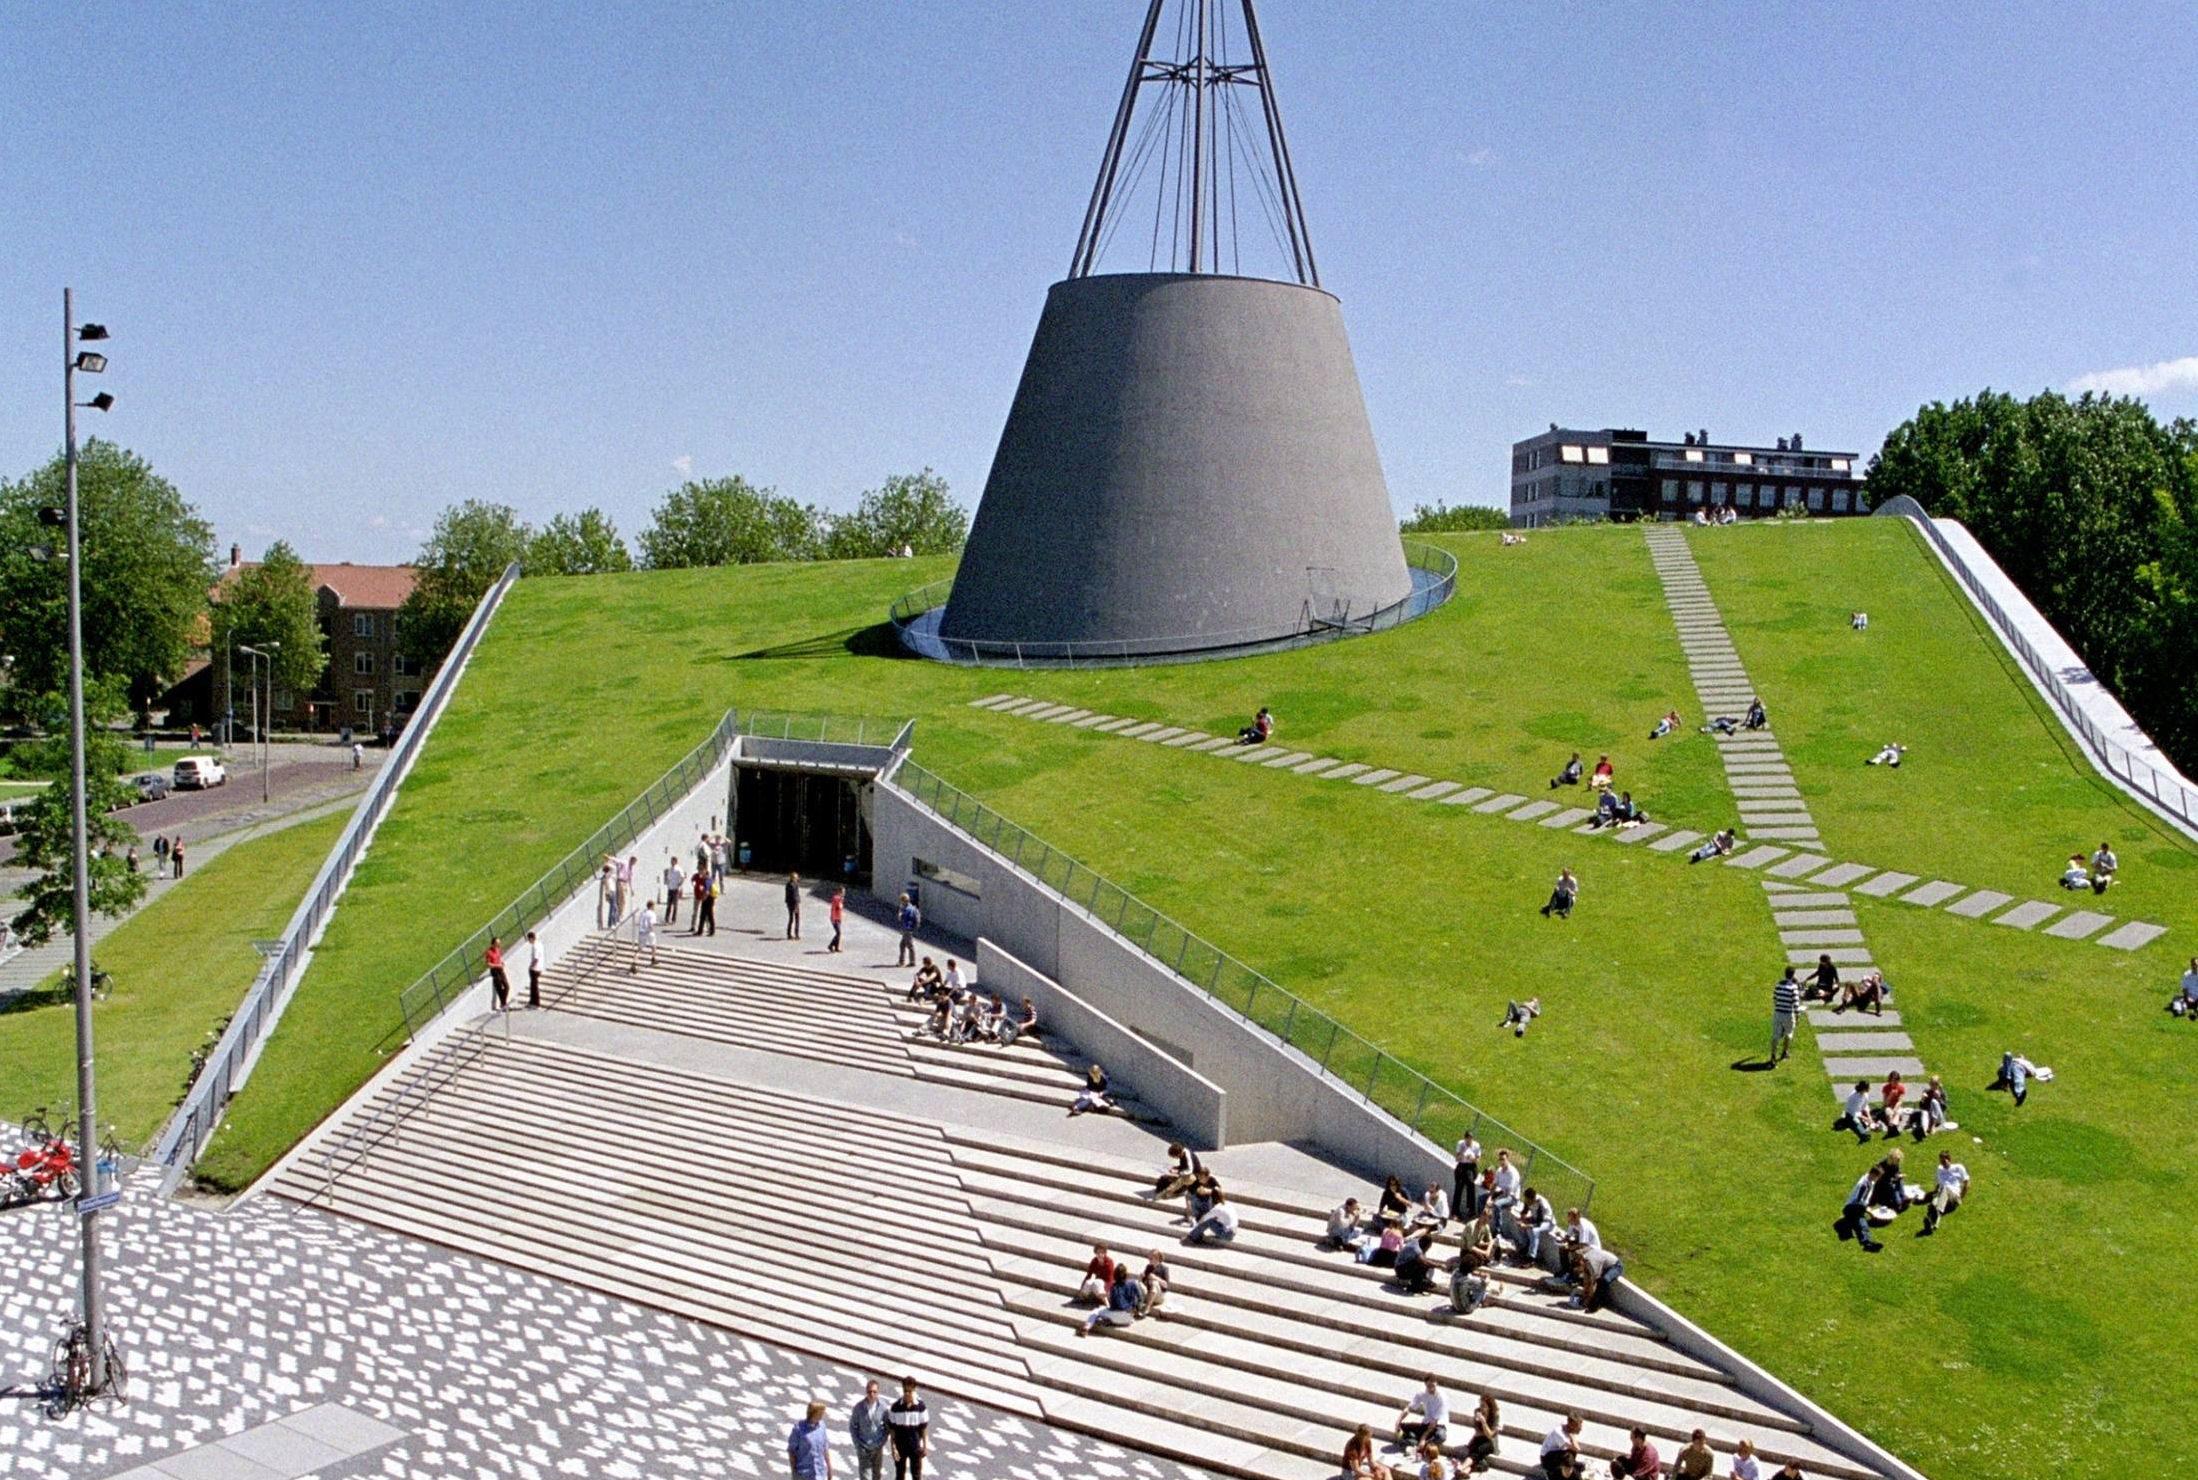
\includegraphics[width=\paperwidth,height=\paperheight]{images/background-titlepage.jpg}}%
\setbeamertemplate{footline}{\usebeamertemplate*{minimal footline}}
\frame{\titlepage}
}

{\setbeamertemplate{footline}{\usebeamertemplate*{minimal footline}}
\begin{frame}\frametitle{\titleTOC}
	\tableofcontents
\end{frame}
}

\section{Project Description}
\subsection{Project Overview}

\begin{frame}\frametitle{Project Overview}
	%\begin{example}
		%\begin{minipage}{0.6\textwidth}
			% insert picture (pdf file)
			%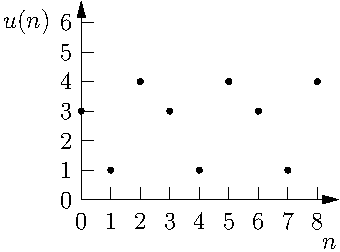
\includegraphics{images/ex1_periodic_number.pdf}
		%\end{minipage}
		%\centering{$u(n)=[3,1,4]_n$}
	%\end{example}
	
	\begin{figure}[H]
	\begin{minipage}[t]{0.45\textwidth}
	\centering
	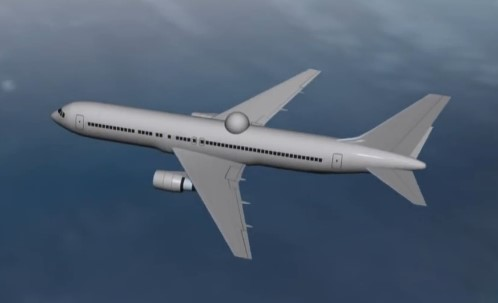
\includegraphics[width=\linewidth]{images/past_antenna}
	\caption{Mechanical Antenna on Aeroplane}
	\label{fig:past_antenna}
	\end{minipage}
	\hspace{\fill}
	\begin{minipage}[t]{0.45\textwidth}
	\centering
	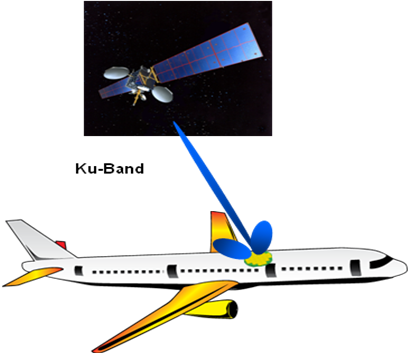
\includegraphics[width=\linewidth]{images/satrax_plane}
	\caption{Phased Array Antennas on Aeroplane}
	\label{fig:satrax_plane}
	
	\end{minipage}
	\end{figure}
	
\end{frame}

\begin{frame}\frametitle{Project Overview}
	\begin{figure}[H]
		\begin{minipage}[t]{0.45\textwidth}
			\centering
			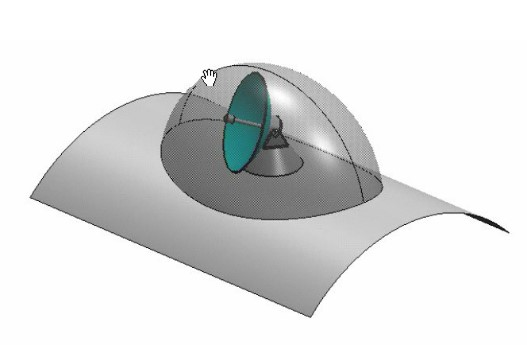
\includegraphics[width=\linewidth]{images/past_antenna1}
			\caption{Mechanical antenna}
			\label{fig:past_antenna1}
		\end{minipage}
			\hspace{\fill}
		\begin{minipage}[t]{0.45\textwidth}
			\centering
			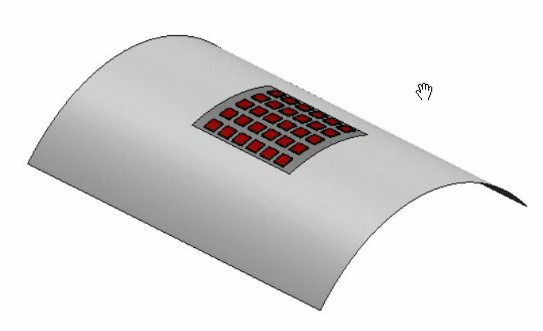
\includegraphics[width=\linewidth]{images/paa_1}
			\caption{Phased array antennas}
			\label{fig:paa_1}
		\end{minipage}
	\end{figure}
\end{frame}

\subsection{Phased Array Antennas}

\begin{frame}\frametitle{Phased Array Antennas}
		\begin{figure}
			\centering
			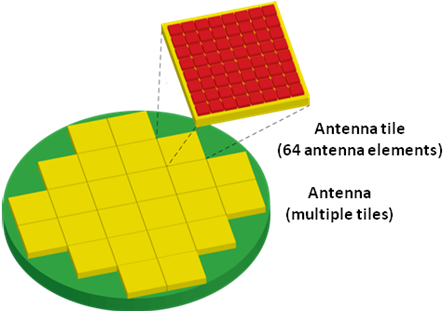
\includegraphics[width=0.3\linewidth]{images/satrax_antenna}
			\caption{PAA configuration}
			\label{fig:satrax_antenna}
		\end{figure}
		\begin{figure}[H]
			\begin{minipage}[t]{0.45\textwidth}
				\centering
				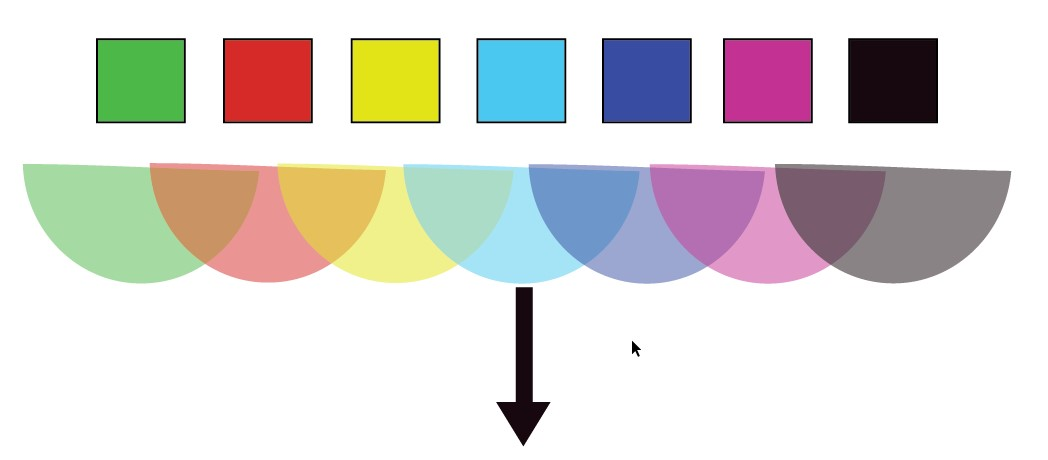
\includegraphics[width=\linewidth]{images/paa_straight}
				%\caption{Delay control of PAA }
				%\label{fig:bandwidth1}
			\end{minipage}
				\hspace{\fill}
			\begin{minipage}[t]{0.45\textwidth}
				\centering
				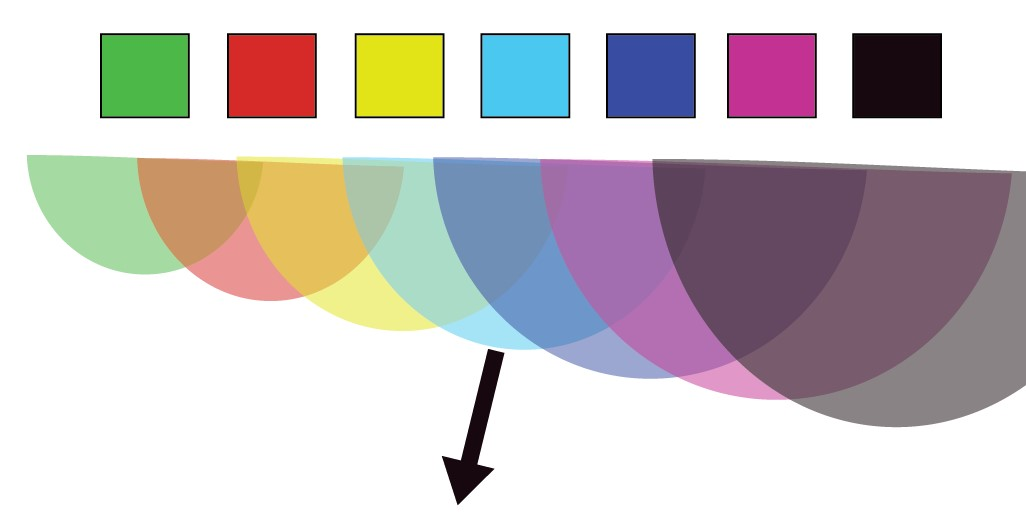
\includegraphics[width=\linewidth]{images/paa_bend}
				%\caption{Delay estimation}
				%\label{fig:bandwidth2}
			\end{minipage}
		\end{figure}
\end{frame}

\subsection{OBFN Chip}

\begin{frame}\frametitle{OBFN Chip}
		\begin{figure}
			\centering
			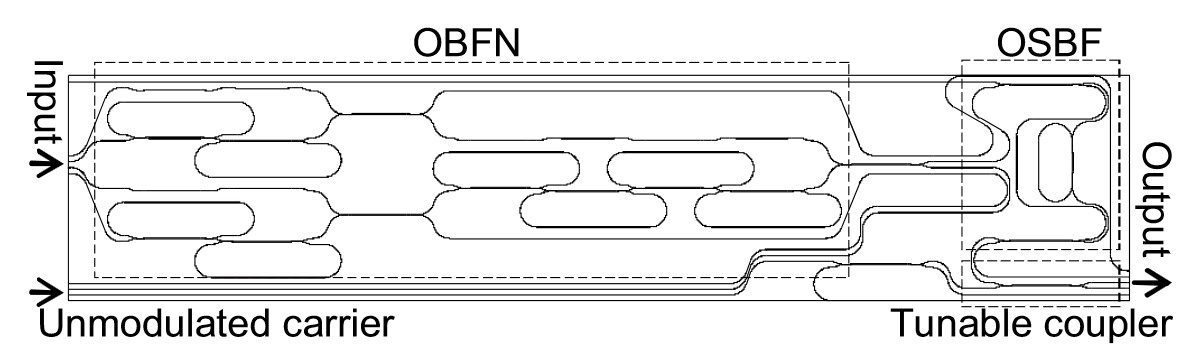
\includegraphics[width=0.8\linewidth]{images/OBFN_chip}
			\caption{Waveguide layout of an integrated beamformer chip}
			\label{fig:OBFN_chip}
		\end{figure}
\end{frame}

\subsection{Optical Ring Resonator (ORR)}

\begin{frame}\frametitle{Optical Ring Resonator (ORR)}
	\begin{figure}[H]
			\begin{minipage}[t]{0.4\textwidth}
				\centering
				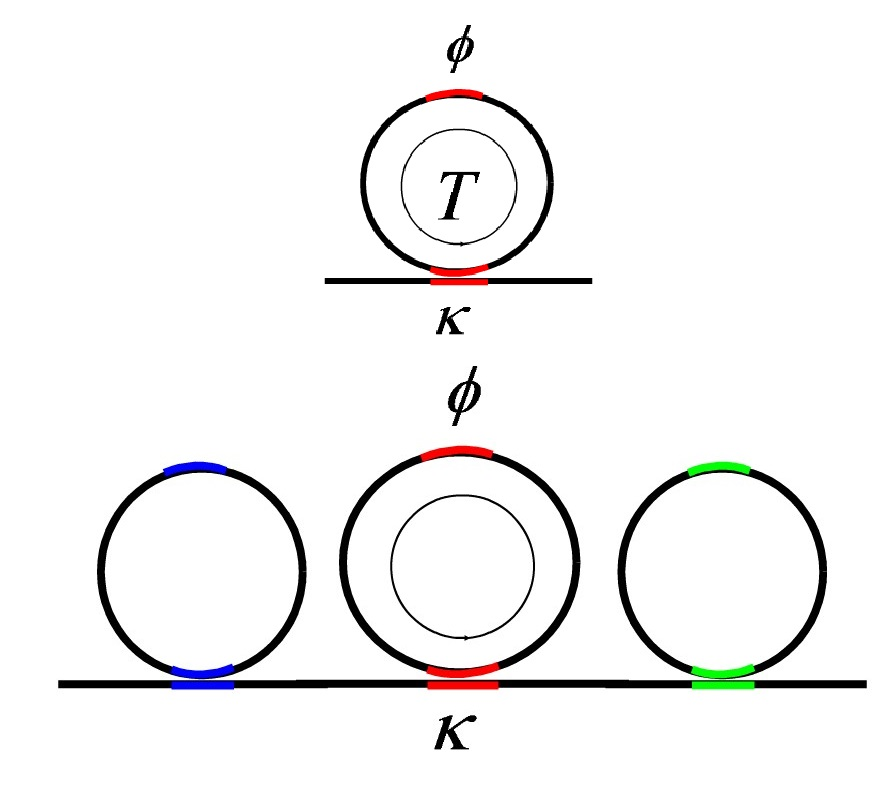
\includegraphics[width=\linewidth]{images/ORR}
				\caption{Optical Ring Resonator Configuration}
				\label{fig:ORR}
			\end{minipage}
				\hspace{\fill}
			\begin{minipage}[t]{0.55\textwidth}
				\centering
				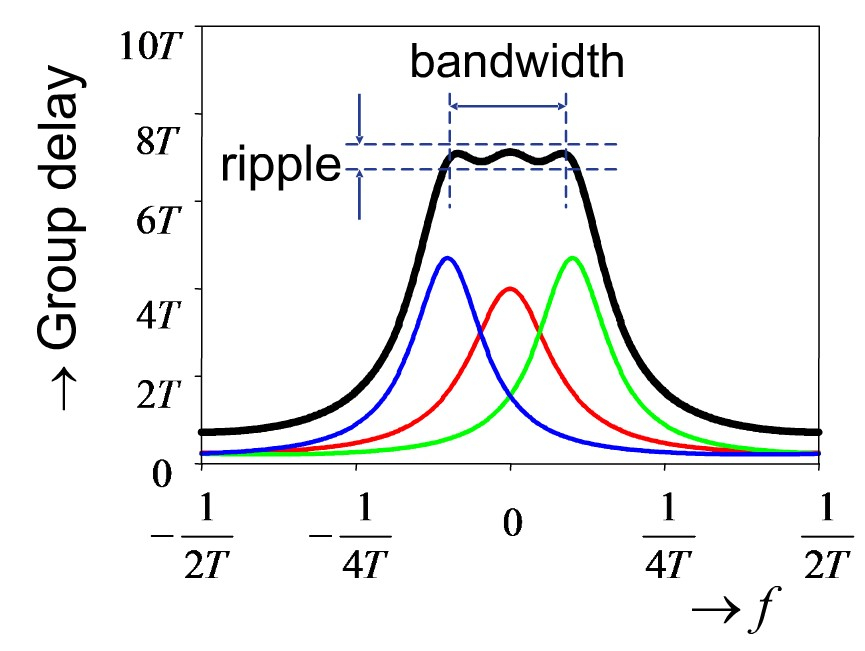
\includegraphics[width=\linewidth]{images/ORR2}
				\caption{Delay, ripple, and bandwidth graph}
				\label{fig:ORR2}
			\end{minipage}
	\end{figure}
\end{frame}

\section{Tuning of OBFN}

\subsection{Parameter to be Tuned}

\begin{frame}\frametitle{Parameters to be Tuned}

	\begin{figure}
			\centering
			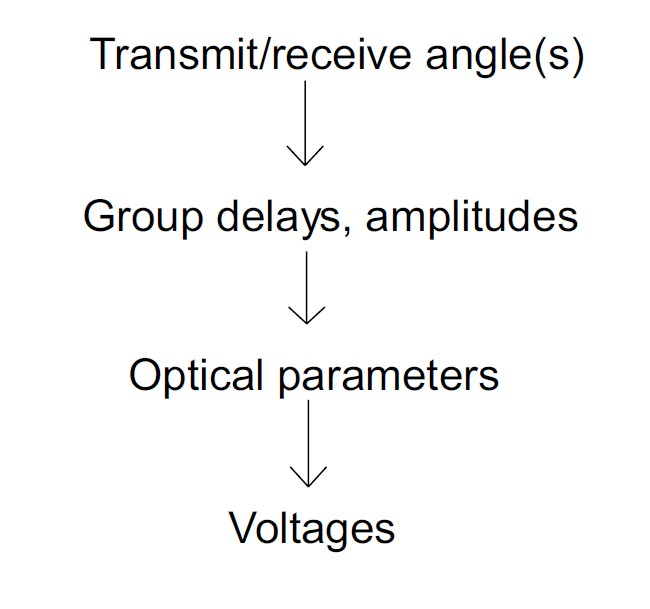
\includegraphics[width=0.4\linewidth]{images/project_layer}
			%\caption{The Project layers}
			%\label{fig:projlayers}
	\end{figure}
	\begin{block}{Parameters to be Tuned: Optical Parameters}
		Parameters to be tuned to get the desired goals are the optical parameters : $\kappa$, $\phi$, and $T$ of each ORR\\
	\end{block}
\end{frame}

\subsection{Desired Goals of Tuning}

\begin{frame}\frametitle{Desired Goals of Tuning}
	\begin{figure}
			\centering
			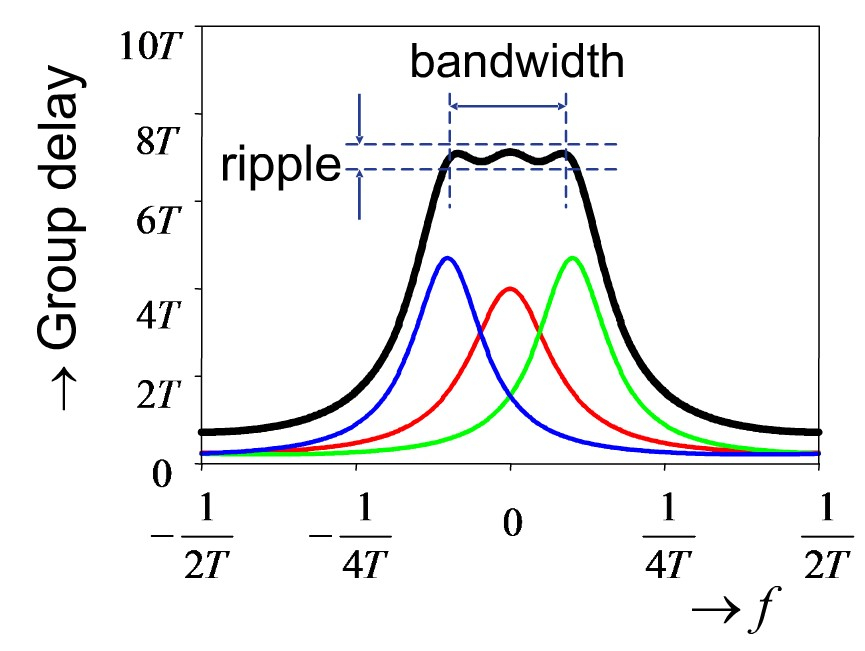
\includegraphics[width=0.45\linewidth]{images/ORR2}
			%\caption{The Project layers}
			\label{fig:projlayers}
	\end{figure}
	\begin{block}{Goals: Group delays, ripple and bandwidth}
		\begin{itemize}
		\item \textbf{Group delays} : a certain value, depends on the angle of signal\\
		\item \textbf{Ripple} : flat\\
		\item \textbf{Bandwidth} : alligned with the spectrum of the modulated optical signal
		\end{itemize}
	\end{block}
\end{frame}

\begin{frame}\frametitle{Desired Goals of Tuning}
	\begin{figure}
			\centering
			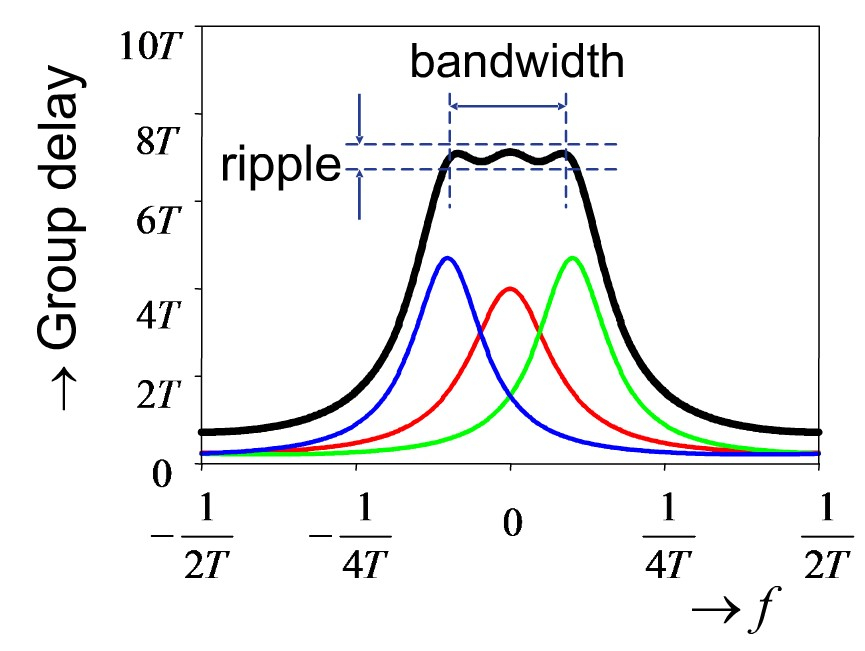
\includegraphics[width=0.45\linewidth]{images/ORR2}
			%\caption{The Project layers}
			\label{fig:projlayers}
	\end{figure}
	\begin{alertblock}{Tradeoff!}
		There is a \textbf{tradeoff} between the group delays, ripple, bandwidth and the number of ORR needed.
	\end{alertblock}
\end{frame}

\subsection{Tuning Methods}

\begin{frame}\frametitle{Tuning Methods - NLP}
	\begin{definition}
		Search for the parameters that minimize the cost function $\mu$ subject to several constraints.\\
		The usual notation of this problem is as follows\\
		\centering
		\begin{tabular}{c}
		
						$\min_{x}\mu(x)$\\
						$s.t$ \\
						$\textbf{l}\leqslant \textbf{x}\leqslant \textbf{u}$\\
						$g_i(x)=0$\\
						$g_i(x)\leqslant 0$\\
		\end{tabular}
	\end{definition}
	
	It is implemented in the $fmincon$ function of MATLAB
	
\end{frame}

\begin{frame}\frametitle{Tuning Methods - NLP - Cost Functions}
	\begin{block}{Delay Criterion}
	Delay Criterion can be used as a cost function.\\
	$$
	\mu = \sum_{k}(\tau_{total}(f_k)-D)^2
	$$
	with\\
	$$
	\tau_l(f)=\frac{\kappa_lT}{2-\kappa_l-2\sqrt{1-\kappa_l}\textup{cos}(2\pi fT+\phi _l)}
	$$
	and $D$ is the desired delay value
	\end{block}
\end{frame}

\begin{frame}\frametitle{Tuning Methods - NLP - Cost Functions}
	\begin{block}{Phase Criterion}
	Phase Criterion can be used as a cost function.\\
	
	$$
	\mu=\sum_{n}\left ( \psi _{total}(f_0+f_{IF,n}) +2\pi D(f_0+f_{IF,n})\right )^2
	$$
	with\\
	\scriptsize
	$$
	\psi (f)=\arctan\left ( \frac{\sin(2\pi fT+\phi_l)}{\sqrt{1-\kappa_l}-\cos(2\pi fT+\phi_l)}\right )-\arctan\left ( \frac{\sqrt{1-\kappa_l}\sin(2\pi fT+\phi_l)}{1-\sqrt{1-\kappa_l}\cos(2\pi fT+\phi_l)}\right )
	$$
	\normalsize 
	and $D$ is the desired delay value
	\end{block}
\end{frame}

\begin{frame}\frametitle{Tuning Methods - NLP - Cost Functions}
	\begin{block}{Power Criterion}
	Power Criterion can be used as a cost function.\\
	
	$$
	\mu=\sum_{n}\left [ P_{ideal}-P_{actual}\right ]^2
	$$
	with\\
	$$
	P_{ideal}=\sum_{m=1}^{M}a_m\left | H_m(f_o+f_{IF,n}) \right |
	$$\\
	\footnotesize
	$$
	P_{actual}=\left | \sum_{m=1}^{M}a_m\left | H_m(f_o+f_{IF,n}) \right |\exp(j(\psi_{total,m}((f_o+f_{IF,n}))+D_m(f_o+f_{IF,n}))) \right |
	$$\\
	\normalsize 
	and $D_m$ is the desired delay value
	\end{block}
\end{frame}

\subsection{Proposed Tuning Methods - Machine Learning}

\begin{frame}\frametitle{Proposed Tuning Methods - Machine Learning}
	\begin{definition}
		Machine learning concept can be used to train the neural networks to get the optimum parameters which minimize the error (cost function $\mu$)
		
	\end{definition}
	Cost function $\mu$ that can be used is Power Criterion because it is measurable so it is easy to be compared to the desired one.	
\end{frame}

\section{Machine Learning Tuning Parameters}

\subsection{Cost Function}
	\begin{frame}\frametitle{Cost Functions}
	\begin{block}{Power Criterion}
	Power Criterion can be used as a cost function.\\
	
	$$
	\mu=\sum_{n}\left [ P_{ideal}-P_{actual}\right ]^2
	$$
	or, for mathematical convenience, following $\mu$ can be used\\
	$$
	\mu=\sum_{n}\frac{1}{2}\left [ P_{ideal}-P_{actual}\right ]^2
	$$
	\end{block}
\end{frame}

\subsection{Parameter Gradients}
	\begin{frame}\frametitle{Parameter Gradients}
	\begin{definition}
	The gradient is necessary to determine in which direction will the optimization process go. Since the cost function is an error function of the desired and actual result, the gradient needed is a rate of change of error w.r.t change of parameters.\\
	In machine learning concept, Backpropagation algorithm can be used to find the rate of change of error w.r.t change of parameters.
	\end{definition}
\end{frame}

\subsection{Input and Output of Neural Network}
	\begin{frame}\frametitle{Input and Output of Neural Network}
	\begin{definition}
	Input can be the desired value of power.\\
	Output can be the actual value of power produced.\\
	This means the Neural Network that is used is the network that is able to reproduce its input at the output layer.
	This concept is called Autoencoder.
	\end{definition}
\end{frame}

\subsection{Dropout Regularization}
	\begin{frame}\frametitle{Dropout Regularization}
	\begin{definition}
	One of most common problem in neural network is overfitting, means the system learn over fit to the trained data, which will make the system will not have good result when new test data is introduced.\\
	This problem is handled by a stochastic training method called Dropout regularization.
	\end{definition}
\end{frame}

\end{document}
